\newpage
\appendice{Графический материал}
\label{app:drawings}


\hfill \break
\hfill \break
\hfill \break
~
\rotatebox{90}{\begin{minipage}[b]{0.75\textheight}
\centering
    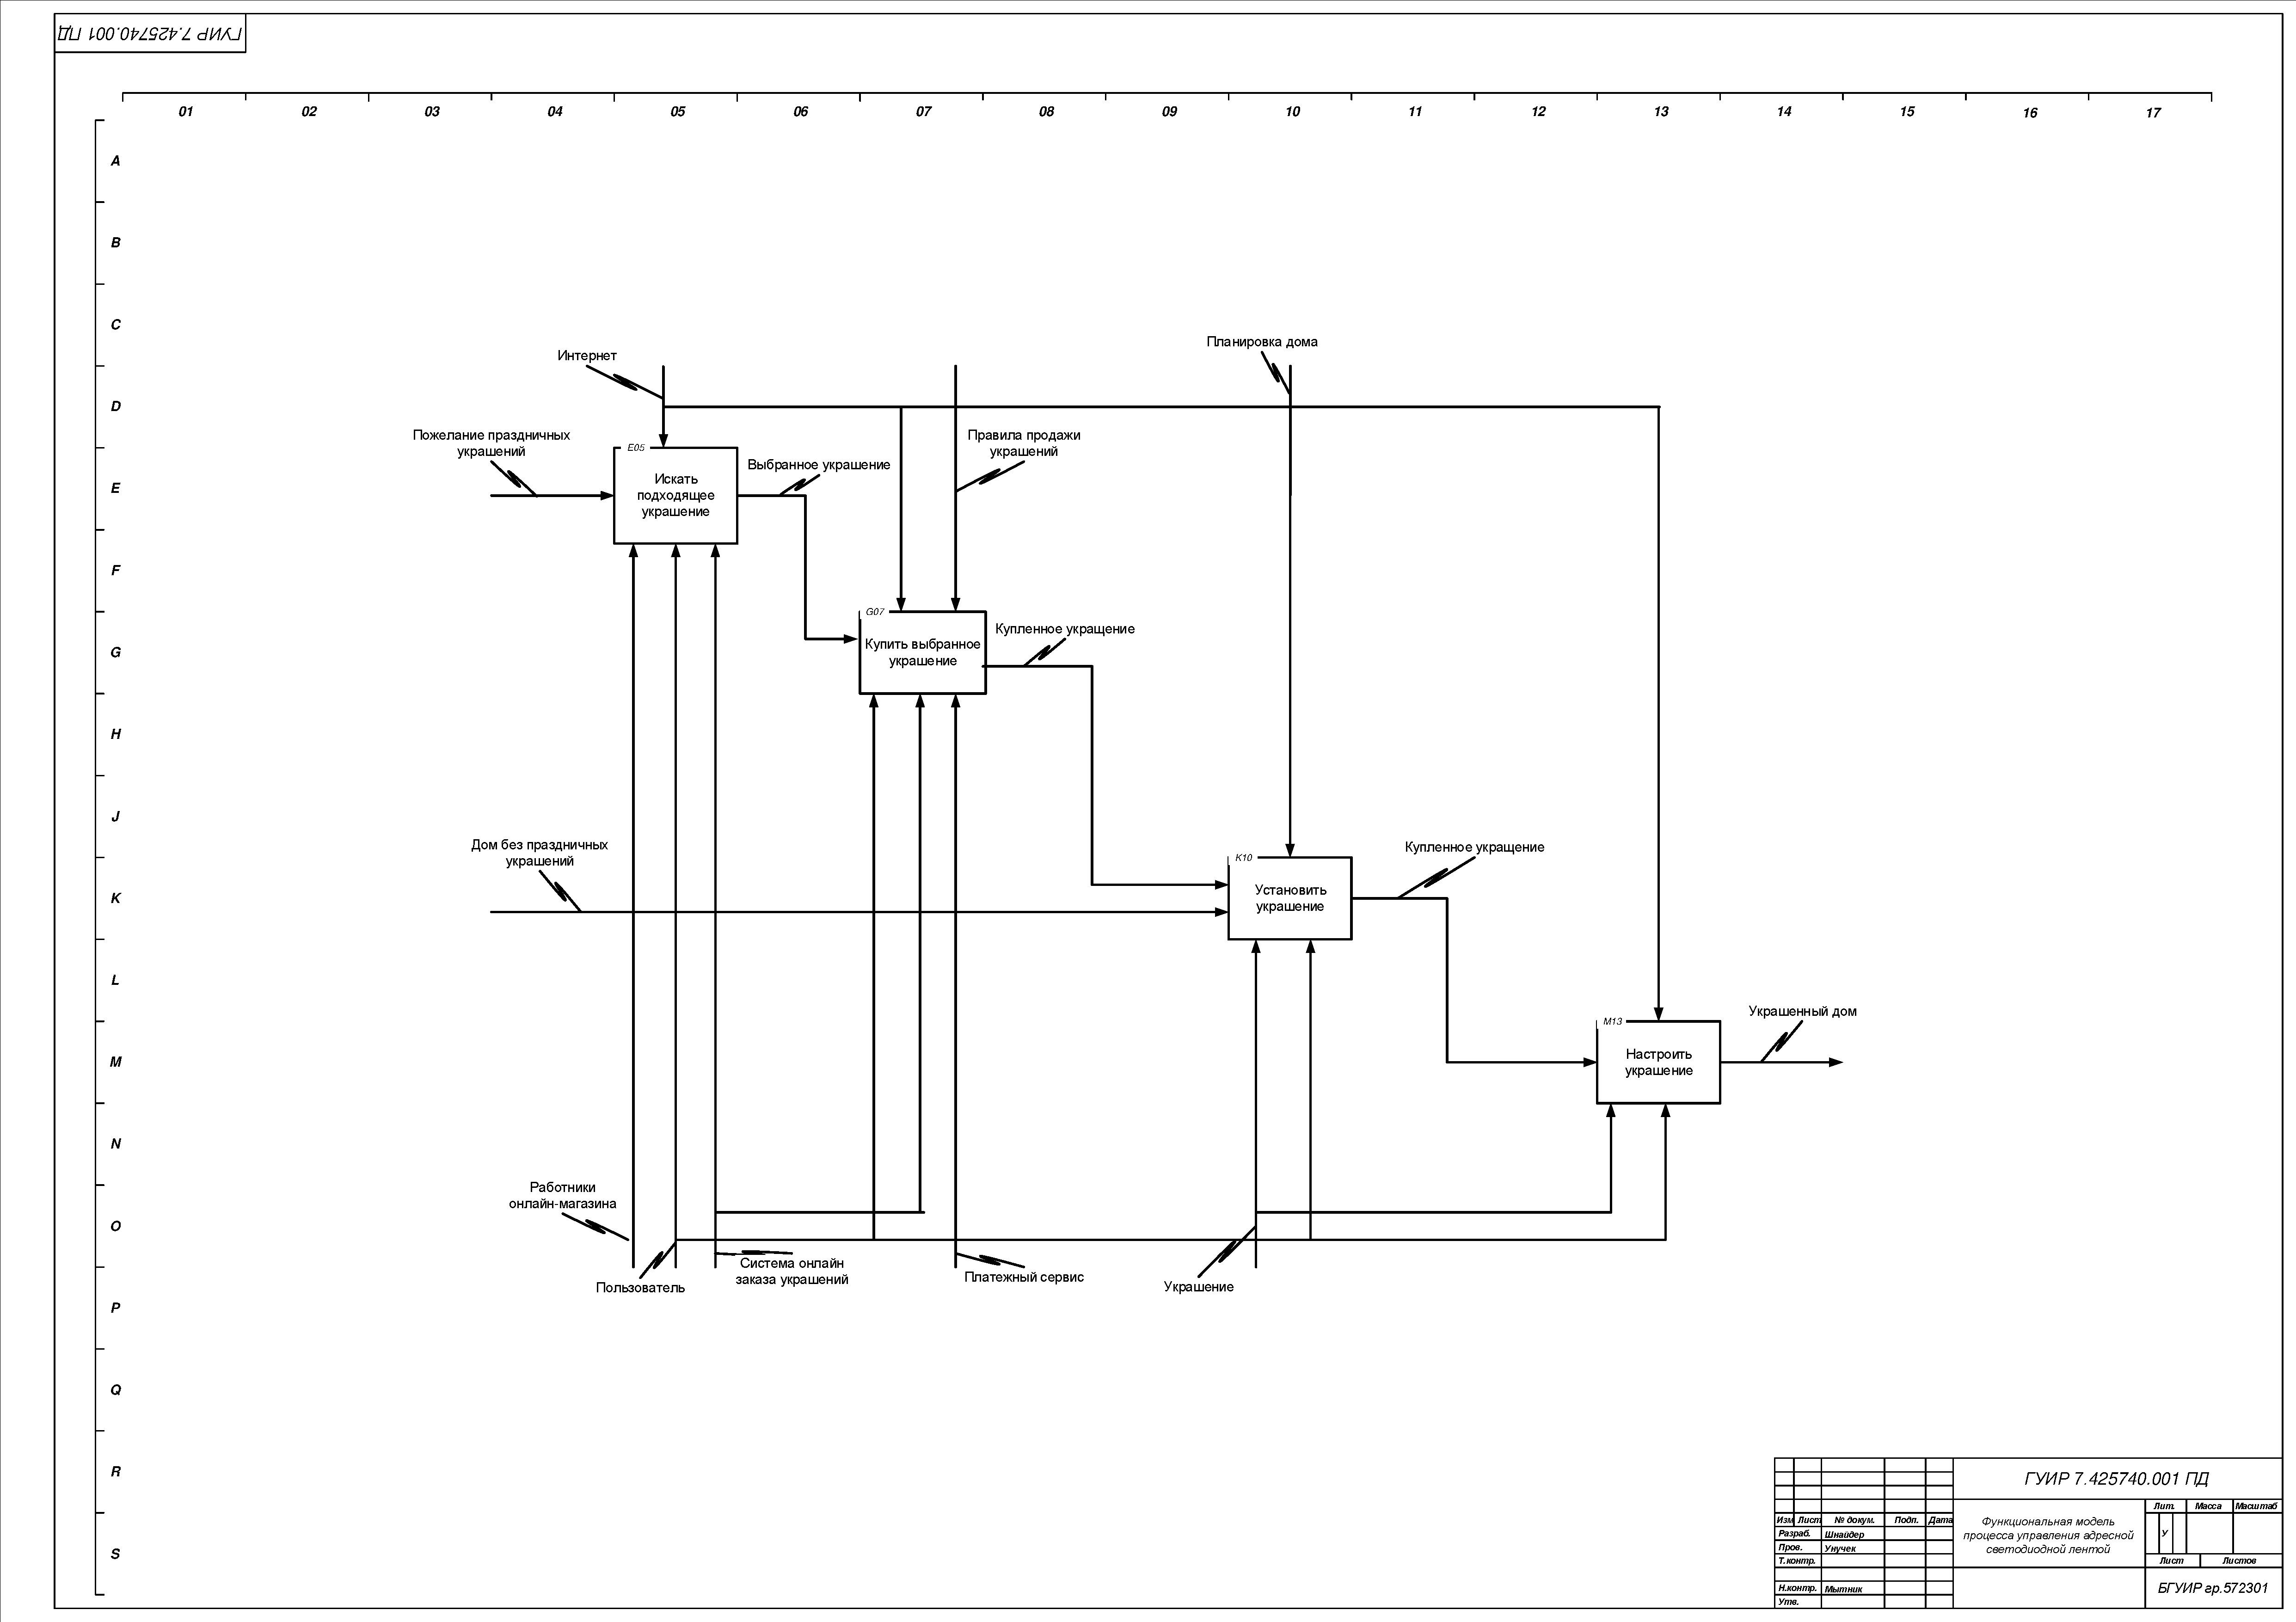
\includegraphics[width=1.1\textwidth]{figures/drawings/drawing_idef0.pdf}
    \captionof{figure}{Функциональная модель процесса управления адресной светодиодной лентой}
    \label{fig:appendices:drawings:approximation}
\end{minipage}}
\newpage
\hfill \break
\hfill \break
\hfill \break
~
\rotatebox{90}{\begin{minipage}[b]{0.75\textheight}
    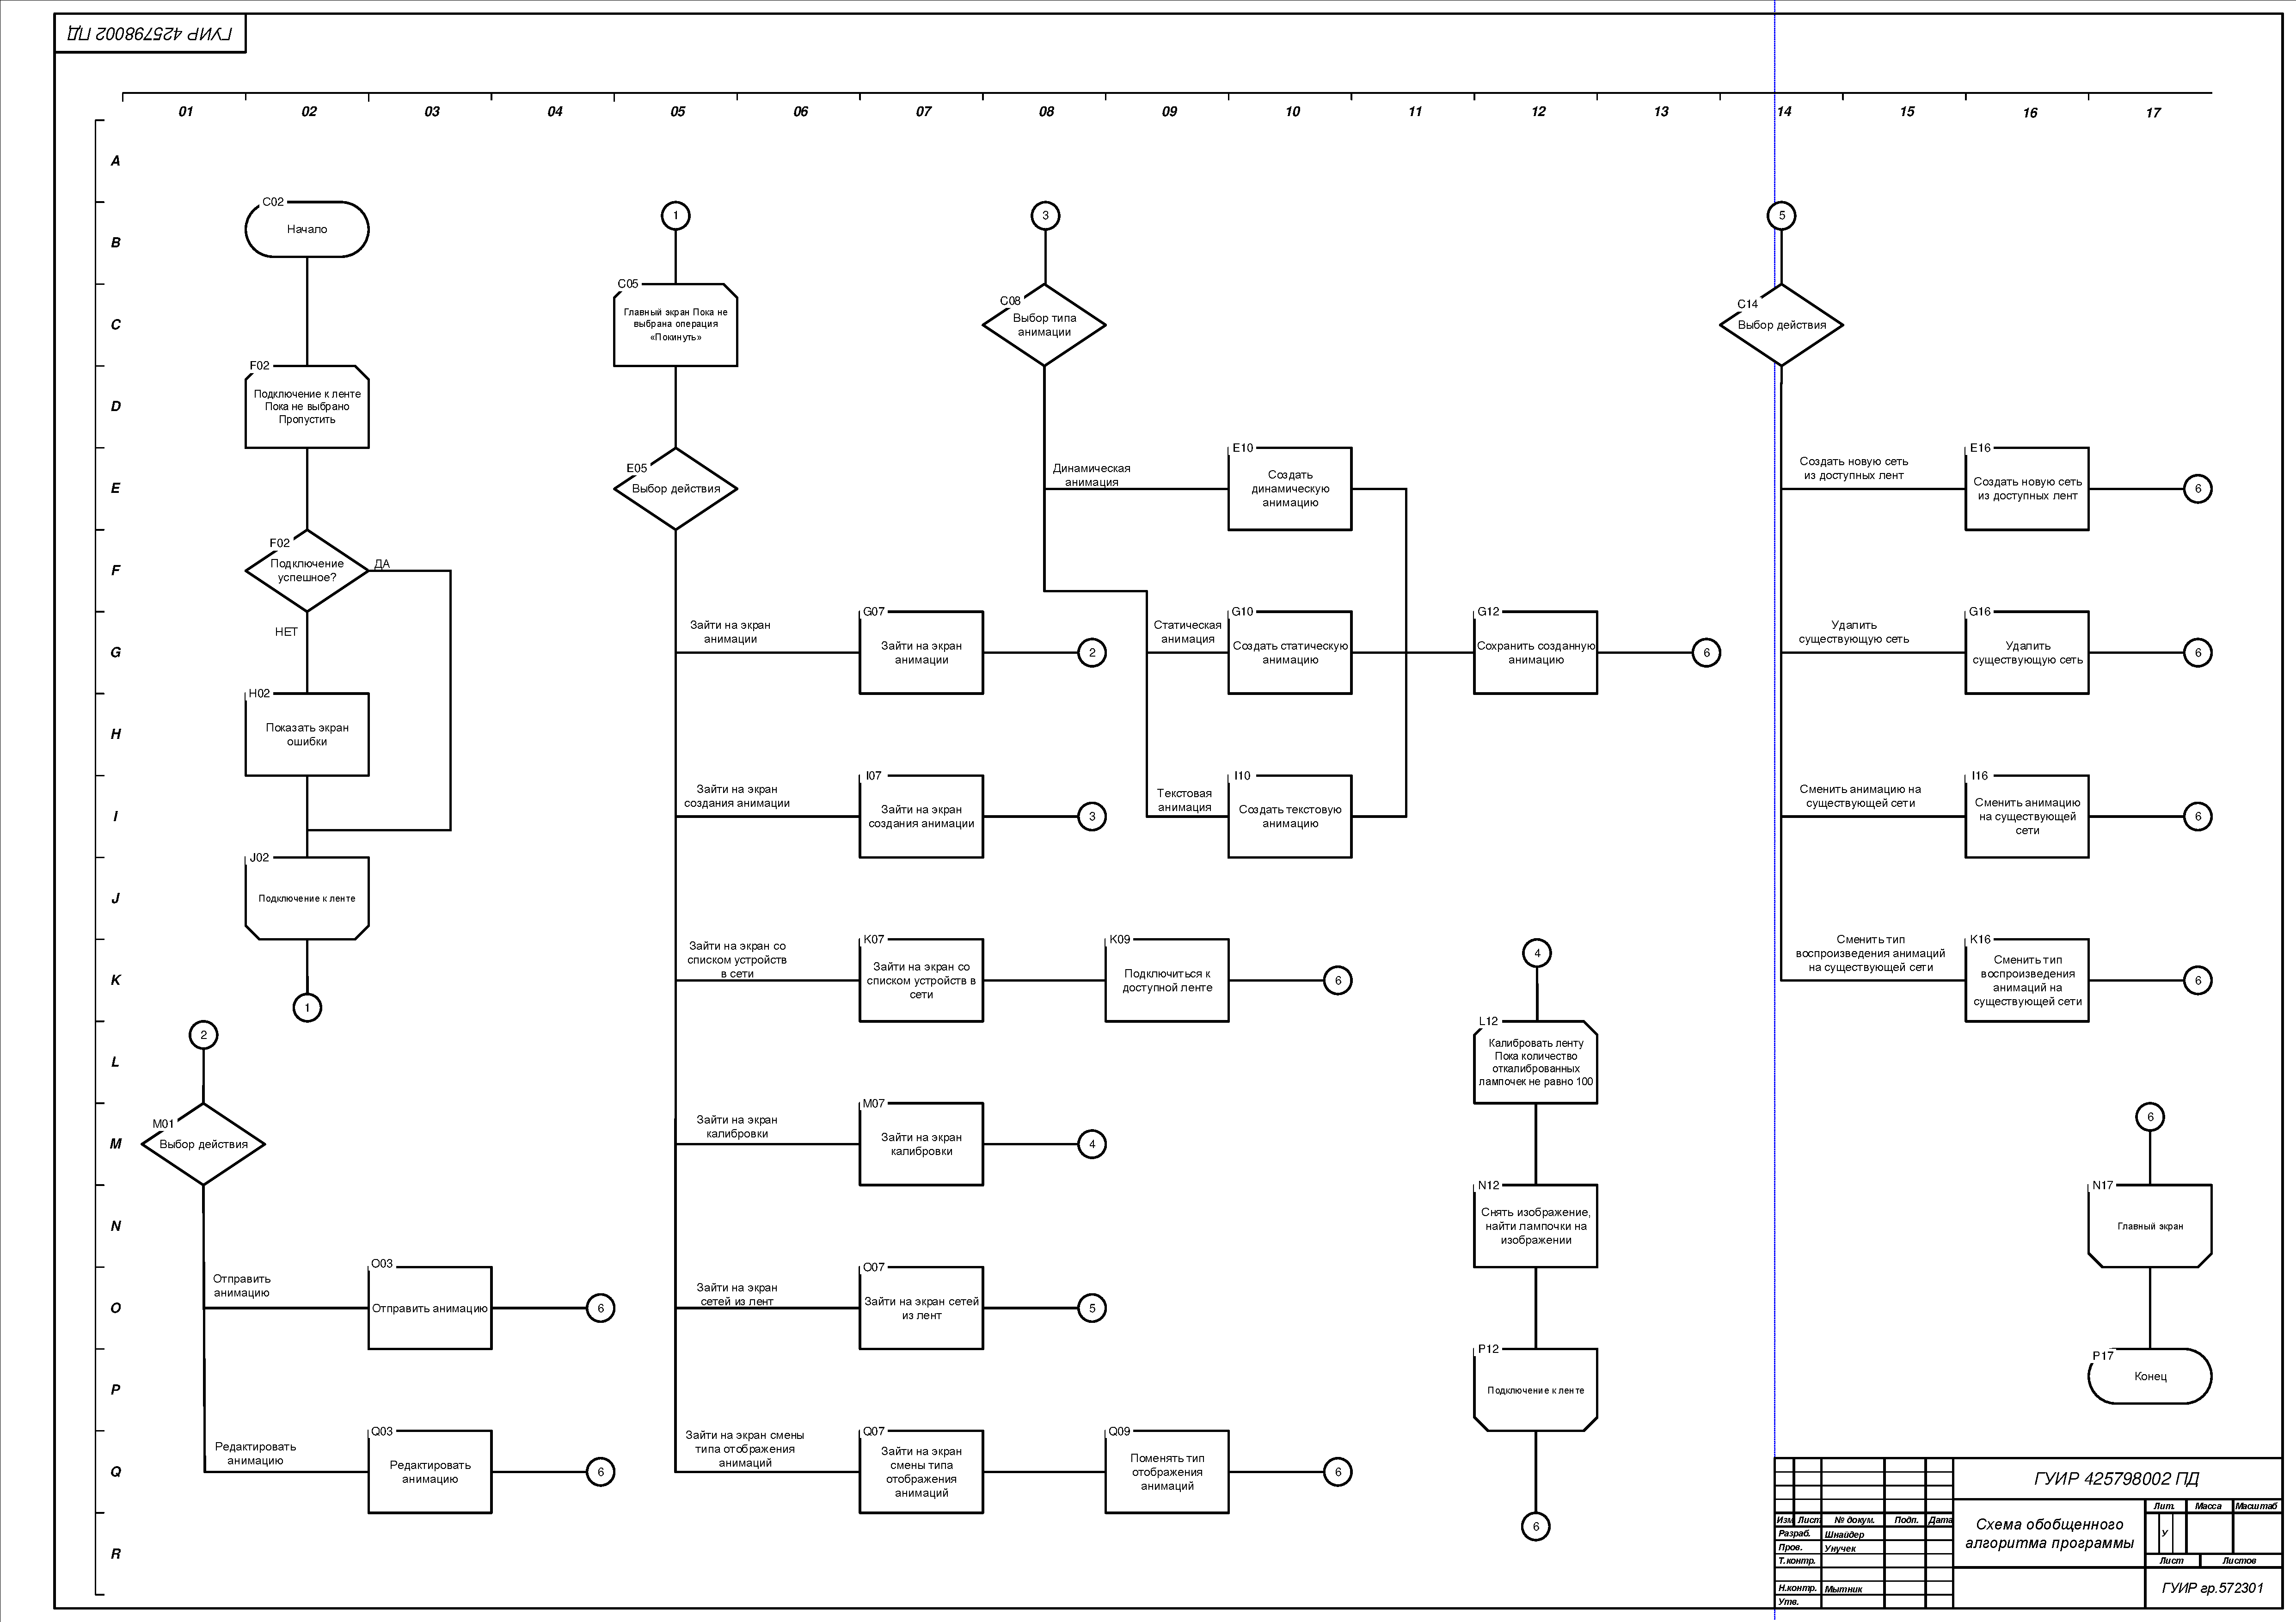
\includegraphics[width=1.1\textwidth]{figures/drawings/drawing_algorithm.pdf}
    \captionof{figure}{Схема обобщенного алгоритма программы}
    \label{fig:appendices:drawings:drawing_algorithm}
\end{minipage}}
~
\begin{figure}[H]
\centering
	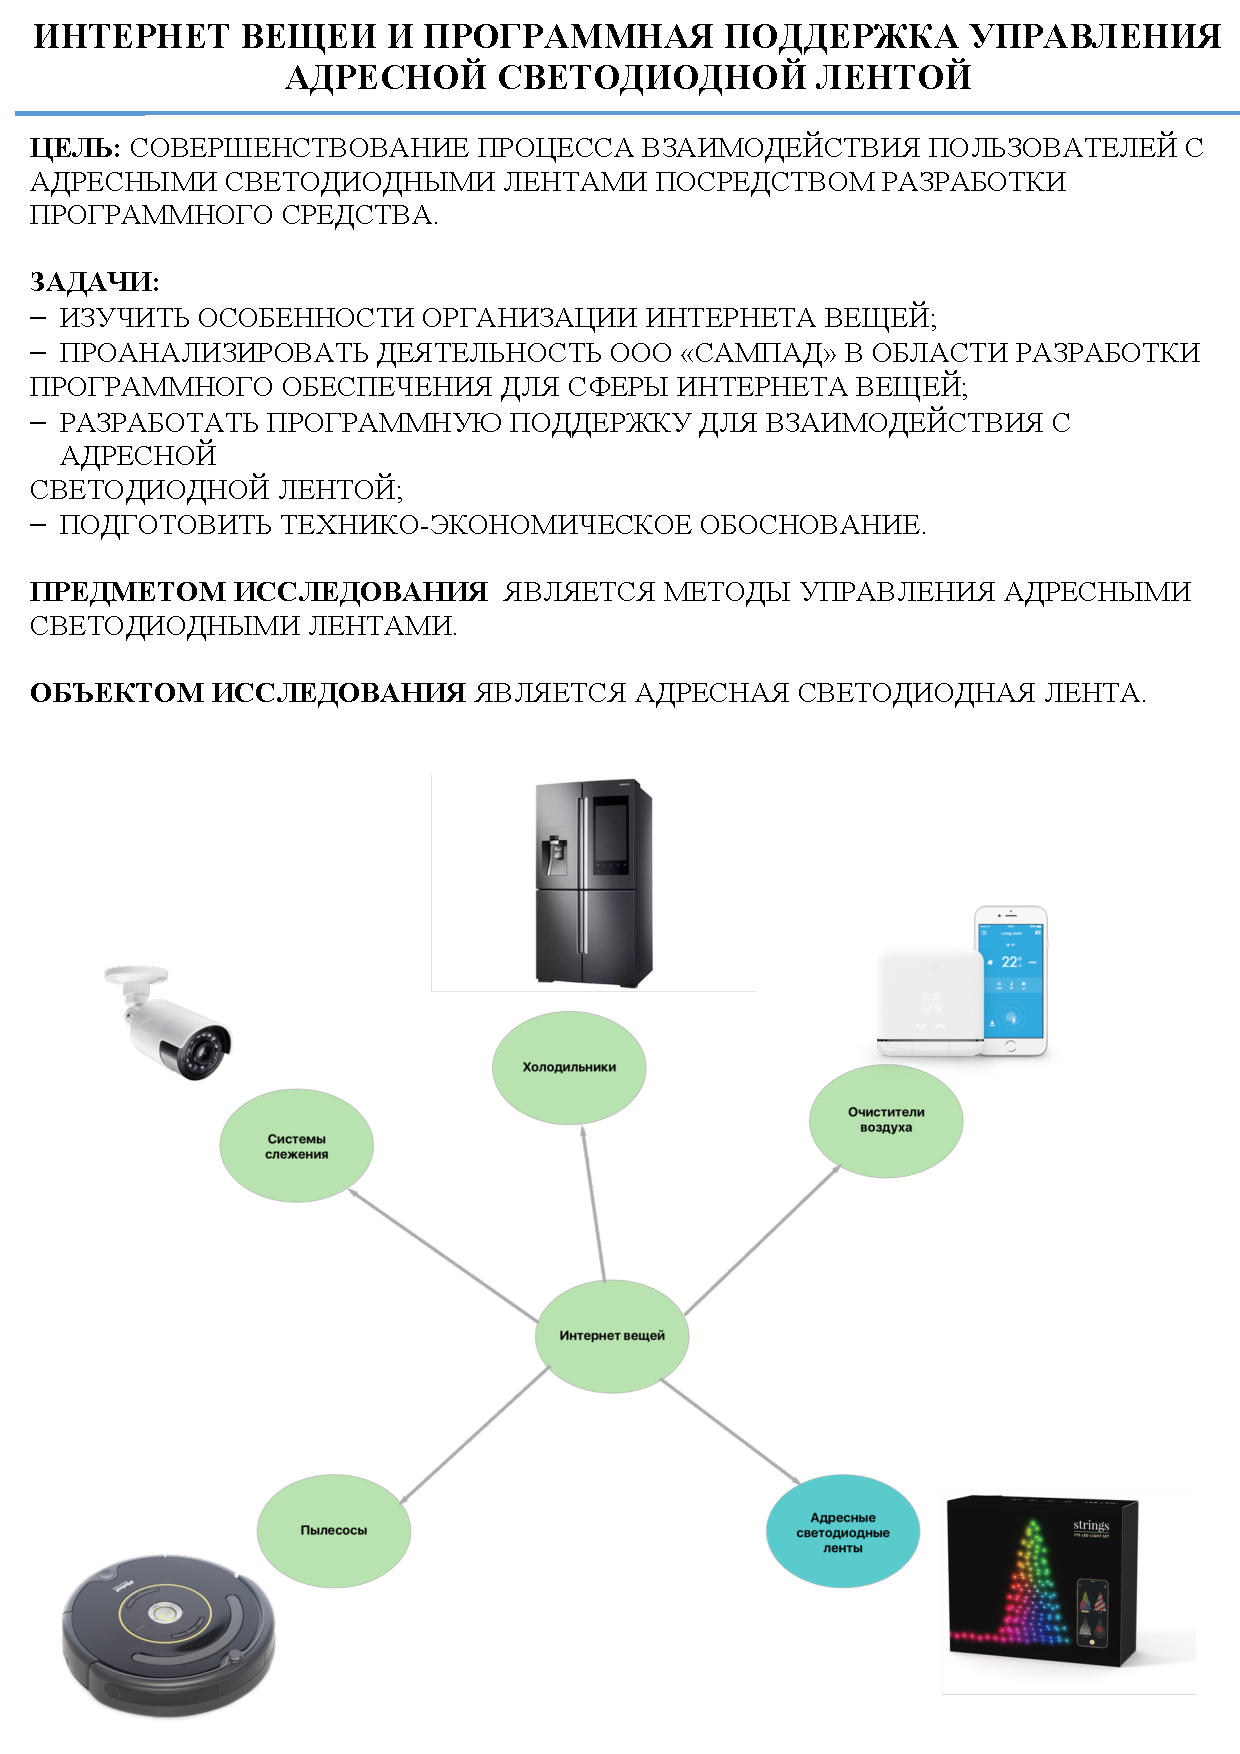
\includegraphics[scale=0.8]{figures/drawings/poster_1.pdf}
	\caption{Плакат Интернет вещей и программная поддержка управления адресной светодиодной лентой}
	\label{fig:appendices:drawings:poster_1}
\end{figure}
\begin{figure}[H]
\centering
	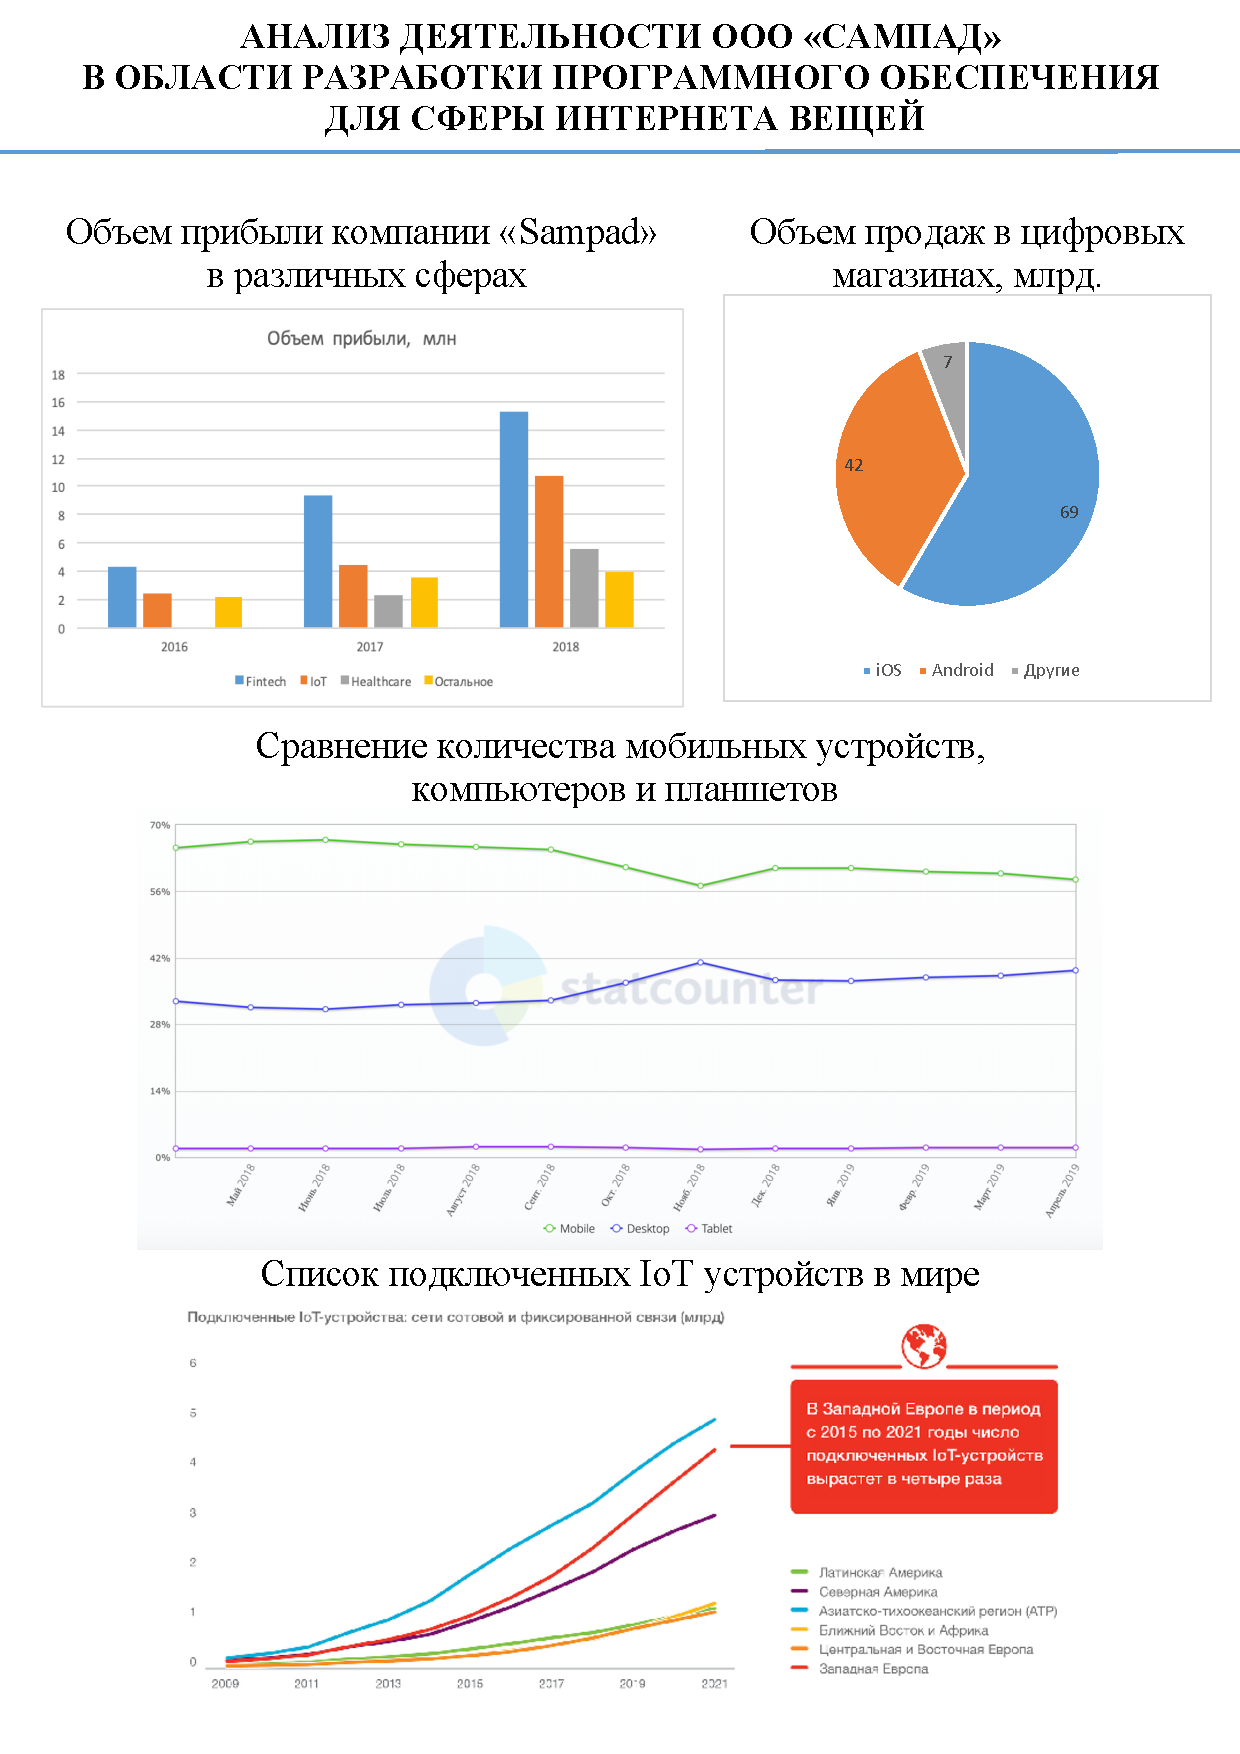
\includegraphics[scale=0.8]{figures/drawings/poster_2.pdf}
	\caption{Плакат анализ деятельности ООО \enquote{Сампад} в области разработки программного обеспечения для сферы Интернета вещей}
	\label{fig:appendices:drawings:poster_2}
\end{figure}
\hfill \break
\hfill \break
\hfill \break
\hfill \break
\hfill \break
~
\rotatebox{90}{\begin{minipage}[b]{0.75\textheight}
    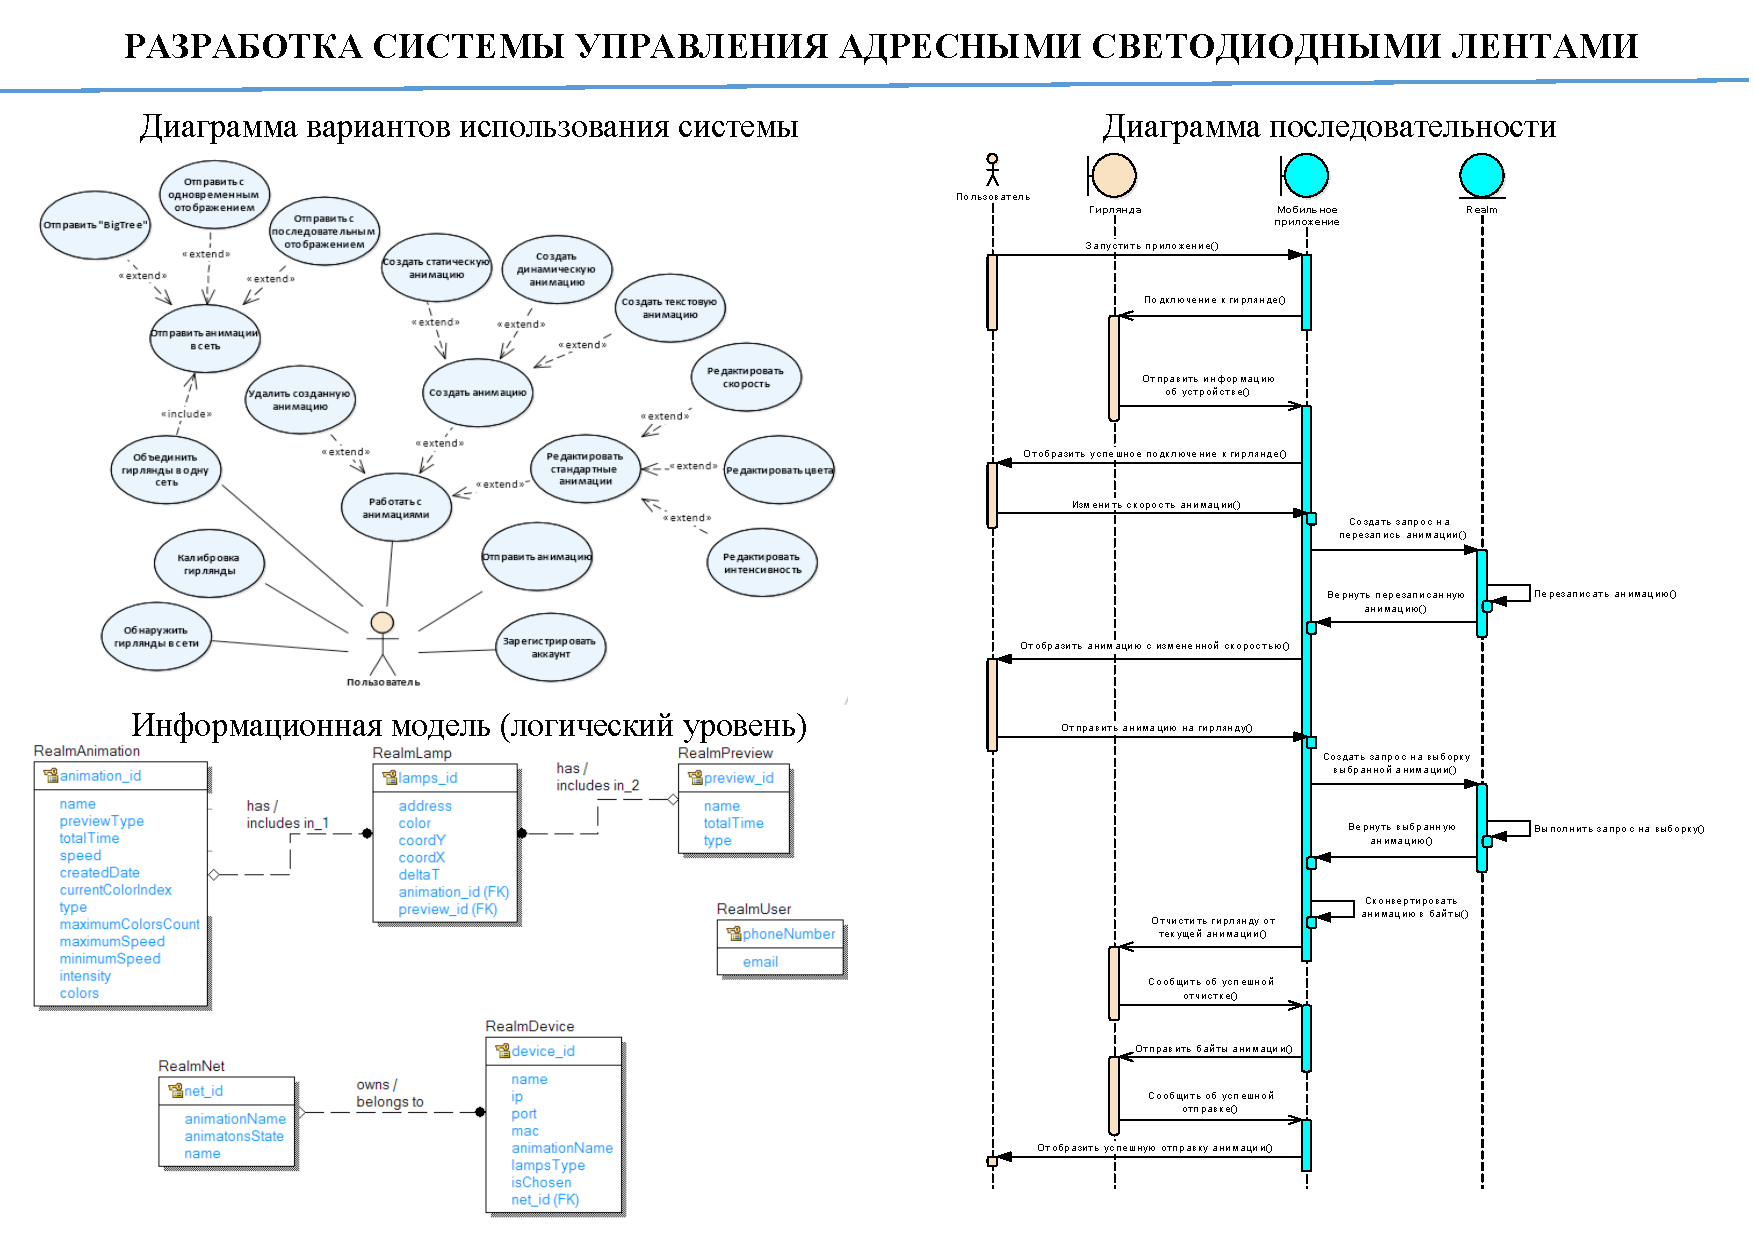
\includegraphics[width=1.1\textwidth]{figures/drawings/poster_3.pdf}
    \captionof{figure}{Плакат разработка системы управления адресными светодиодными лентами}
    \label{fig:appendices:drawings:poster_3}
\end{minipage}}
\newpage
\hfill \break
\hfill \break
\hfill \break
\hfill \break
\hfill \break
~
\rotatebox{90}{\begin{minipage}[b]{0.75\textheight}
    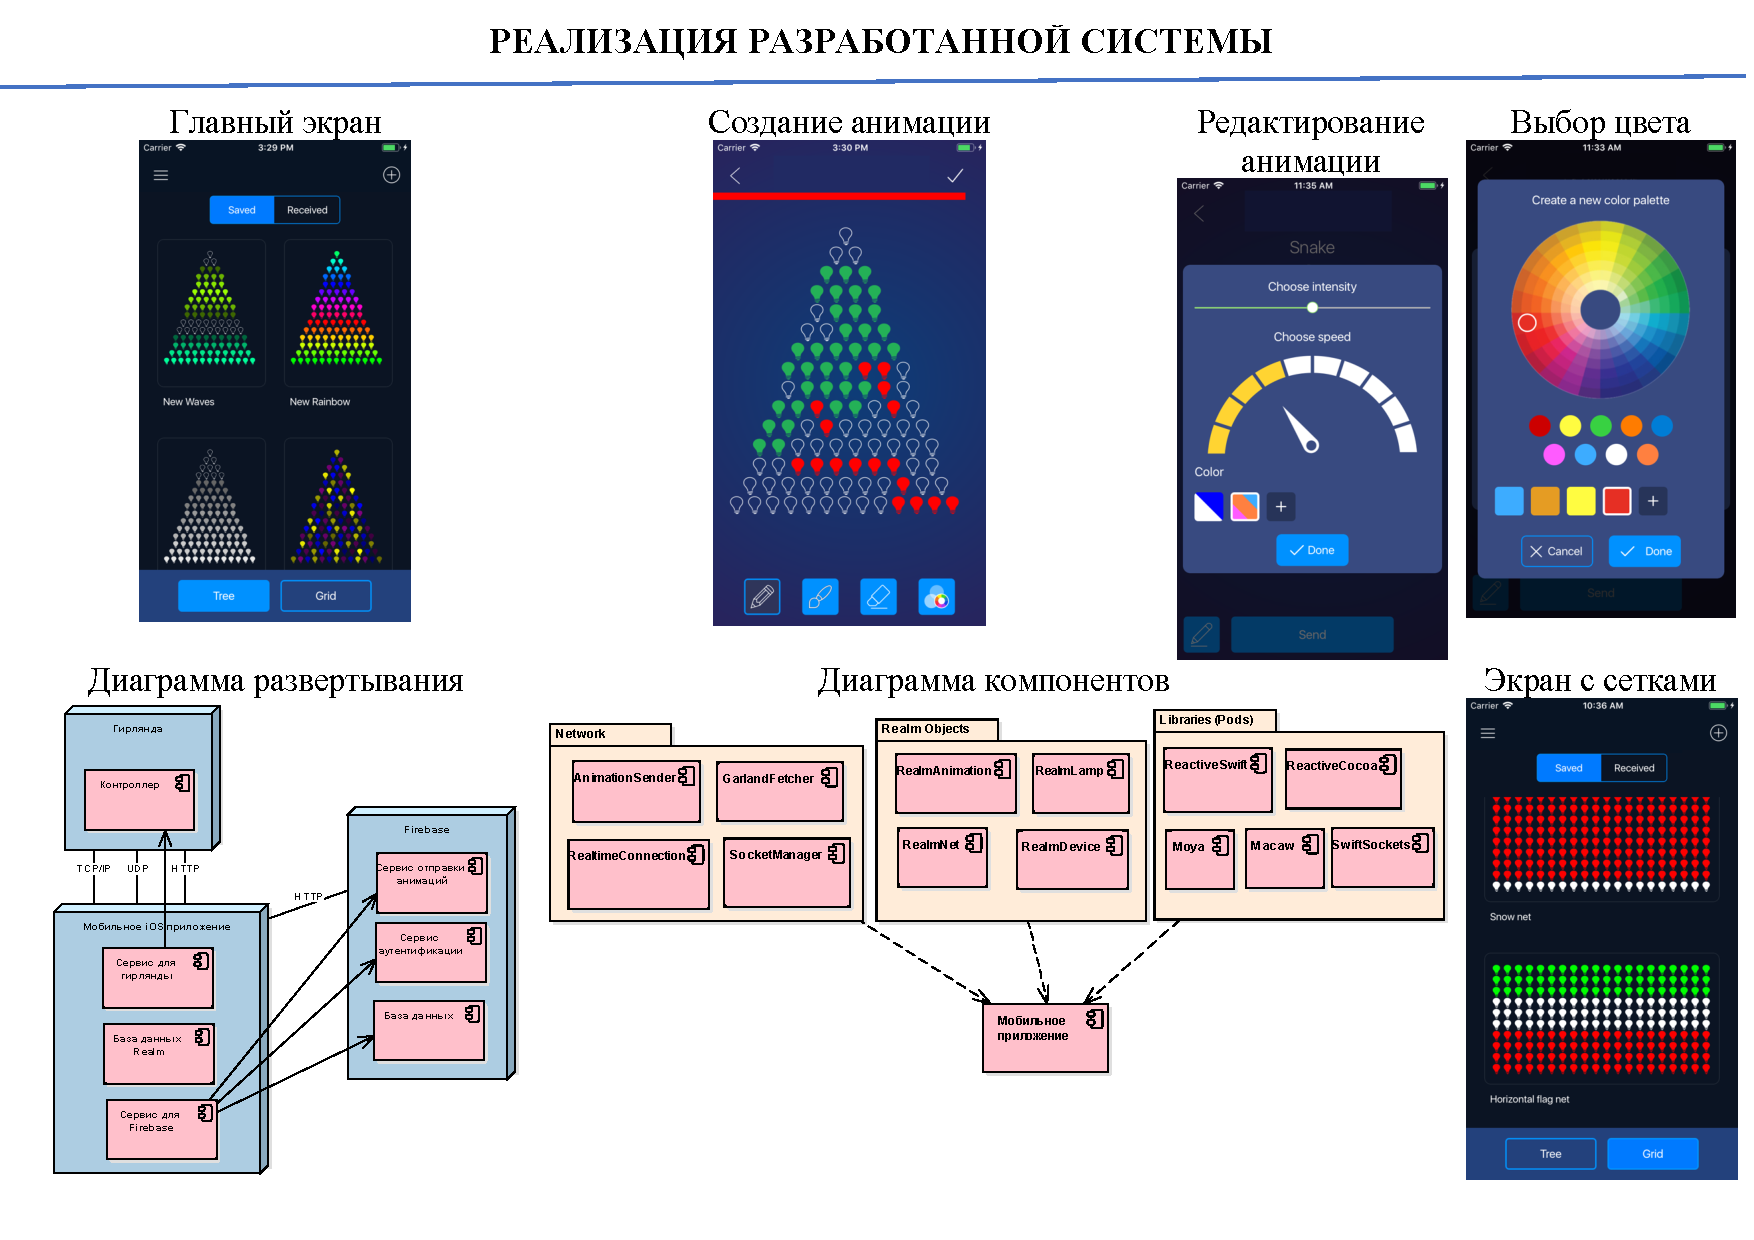
\includegraphics[width=1.1\textwidth]{figures/drawings/poster_4.pdf}
    \captionof{figure}{Плакат реализация разработанной системы}
    \label{fig:appendices:drawings:poster_4}
\end{minipage}}
